%                                                                 aa.dem
% AA vers. 8.2, LaTeX class for Astronomy & Astrophysics
% demonstration file
%                                                       (c) EDP Sciences
%-----------------------------------------------------------------------
%
%\documentclass[referee]{aa} % for a referee version
%\documentclass[onecolumn]{aa} % for a paper on 1 column  
%\documentclass[longauth]{aa} % for the long lists of affiliations 
%\documentclass[rnote]{aa} % for the research notes
%\documentclass[letter]{aa} % for the letters 
%\documentclass[bibyear]{aa} % if the references are not structured 
% according to the author-year natbib style

%
\documentclass[referee]{aa}  
\usepackage[varg]{txfonts}
\usepackage{natbib}
\usepackage{color, colortbl}
\definecolor{LightGray}{gray}{0.8}
\bibpunct{(}{)}{;}{a}{}{,} % to follow the A&A style

%
\usepackage{graphicx}
%%%%%%%%%%%%%%%%%%%%%%%%%%%%%%%%%%%%%%%%
\usepackage{txfonts}
%%%%%%%%%%%%%%%%%%%%%%%%%%%%%%%%%%%%%%%%
%\usepackage[options]{hyperref}
% To add links in your PDF file, use the package "hyperref"
% with options according to your LaTeX or PDFLaTeX drivers.
%

% "to be done"
\usepackage{xcolor}
\newcommand{\tbd}[1]{\textcolor{red}{\textbf{#1}}}


\begin{document} 


   \title{Auroral Radio Source Occultation Modeling and Application to the JUICE Science Mission Planning}
   \titlerunning{Auroral Radio Source Occultation Modeling}
   
   \subtitle{}

   \author{B. Cecconi
          \inst{1}
          \and
          C. Louis\inst{2}
          \and 
          C. Munoz\inst{3}
          \and 
          C. Vallat\inst{3}
          }
    
    
    
   \institute{LESIA, Observatoire de Paris, CNRS, PSL Research University, Meudon, France\\
              \email{baptiste.Cecconi@observatoiredeparis.psl.eu}
         \and
             IRAP, CNRS, Université Paul Sabatier, Toulouse, France\\
             \email{corentin.louis@irap.omp.eu}
         \and
             European Space Agency, ESAC, Madrid, Spain\\
             \email{cmunoz@sciops.esa.int}\\
        \email{cvallat@sciops.esa.int}
             }

   \date{}

% \abstract{}{}{}{}{} 
% 5 {} token are mandatory
 
  \abstract
  % context heading (optional)
  % {} leave it empty if necessary  
   {}
  % aims heading (mandatory)
   {Validate the use of ExPRES as an observation planning tool for the JUICE mission.}
  % methods heading (mandatory)
   {We simulate the occultations of the Jovian auroral radio emissions during the Galileo flybys of the Galilean moons of Jupiter. The ExPRES simulations runs are configured using fixed typical parameters for the main aurora radio emissions. We compare the simulation run results with the actual Galileo PWS observations.}
  % results heading (mandatory)
   {The ExPRES code accurately models the temporal occurrence of the occultations in the whole spectral range observed by Galileo PWS.}
  % conclusions heading (optional), leave it empty if necessary 
   {The method can be applied for preparing the JUICE moon flyby science operation planning.}

   \keywords{Radio emissions --
                Jupiter -- 
                ESA JUICE mission -- 
                ExPRES code
               }

   \maketitle
%
%________________________________________________________________



\section{Introduction} %BC

The magnetosphere of \object{Jupiter} produces low frequency radio emissions from its polar regions, along the active magnetic field lines connected the Jovian auroral oval as well as to the Galilean moon auroral footprints. The Jovian radio emissions are intense and non-thermal radio frequency phenomena, spanning from a few kHz to about 40 MHz, and produced through the Cyclotron Maser Instability (CMI), which converts the local plasma free-energy into electromagnetic radiation \citep{zarka_ASR_92}. They are used as a proxy for the Jovian magnetospheric activity. This radio component has been discovered by \citet{burke_JGR_55} and has been since studied with ground observatories (e.g., in Nan\c cay, France \citep{2017pre8.conf..455L}) and space-borne instruments (with the Voyager, Galileo, Cassini and Juno space missions). 

Observations from the Cassini Radio and Plasma Waves Science (RPWS) \citep{gurnett_SSR_92} and Galileo Plasma Waves Science PWS \citep{gurnett_SSR_92} experiments showed that the Jovian radio emission events are observed quasi-permanently along their orbit. Figure \ref{fig:cas-gll-continuous-radio} shows the observed spectral flux densities by the Cassini/RPWS and Galileo/PWS instruments, during 24 hours, close to the Cassini flyby of Jupiter. Both panels of this figure display many arc-shaped radio events, with a few small time-frequency regions with quiet (background level) conditions. 

\begin{figure}
\includegraphics[width=\linewidth]{figure-gll-cas.pdf}
\caption{Calibrated Cassini/RPWS/HFR \citep{zarka_JGR_04,https://doi.org/10.25935/h98j-ma66} (top) and Galileo/PWS (see Section \ref{gll-pws-data}) (bottom) radio electric power spectral densities during 24 hours close to the Cassini flyby of Jupiter.}\label{fig:cas-gll-continuous-radio}
\end{figure}

Although not covering the full spectral range of the Jovian radio emissions, the PWS (Plasma and Waves Science) investigation \citep{gurnett_SSR_92} of the NASA Galileo mission has routinely collected radio observations during its many orbits in the Jovian system. This data \citep{PWS_LPW_PDS} shows quasi continuous emission from a few 100 kHz up to 5.6 MHz, the upper spectral limit of PWS. During the Galilean moon flybys, Galileo/PWS observed complete occultations of the Jovian radio emissions \citep{Kurth:1997in}.

The ESA JUICE \citep[Jupiter Icy Moon Explorer,][]{2019EPSC...13..400W} will explore the Jupiter system and its magnetosphere. The study of the Jovian magnetosphere can strongly benefit from remote observations and modelling tools \citep{cecconi_baptiste_2019_2583611}. Two instruments of the JUICE scientific payload are operating in the low frequency radio range (below 50 MHz). The Radio and Plasma Waves Instrument (RPWI) has a receiver dedicated to the study of Jovian radio emissions. The Radar for Icy Moon Exploration (RIME) experiment \citep{Bruzzone:2013ge} is operating with a central frequency at 9\,MHz, which lies within the Jovian radio emission spectral range. The Jovian radio emission will interfere with RIME \citep{cecconi_PSS_11} active radar mode, but can be also used in a passive radar experiment mode during icy moon flybys \citep{RomeroWolf:2015fja,Schroeder:2016bu,2017pre8.conf..127K}.

The ExPRES code \citep[Exoplanetary and Planetary Radio Emissions Simulator,][]{Louis_AA_2019} simulates for a given observer the geometrical visibility of radio emissions of a magnetised body. This visibility depends in particular of the emission angle between the magnetic field vector at the source and the emitted wave vector, which is computed self-consistently in the frame of the CMI theory. If the angle between the emitted wave vector and the observer direction, as seen from the source, is lower than the beaming hollow conical sheet width, the emission is seen by the observer. This computation is iterated at each time/frequency step and for each sources. The produced time-frequency map (or dynamic spectrum) can then directly be compared to observations.

In this study, we are modelling the Jovian radio emission occultations during (past) Galileo and (planned) JUICE Galilean moon flybys, using the ExPRES code.  

%__________________________________________________________________

\section{Datasets} %BC
Several datasets have been used in this study and are presented in this section. For the Galileo spacecraft flybys, we compare the actual observed radio flux densities, with low frequency radio occultations predicted by the ExPRES code, using the actual flyby geometry (spacecraft and moon trajectory in a Jovian reference frame). The JUICE spacecraft study only includes modelled occultation.

\subsection{Galileo PWS Observations}
\label{gll-pws-data}
All Galilean moon flyby of Galileo with PWS data have been modelled and analysed. The Galileo PWS (hereafter refered to as GLL/PWS) data have been retrieved from University of Iowa \emph{das2} server interface \citep{piker_2019}, using the \texttt{das2py}\footnote{currently available from \url{https://github.com/das-developers/das2py}} python module. We have used the \emph{Galileo PWS LRS 152-channel calibrated electric} collection\footnote{\url{ http://das2.org/browse?resolve=tag:das2.org,2012:site:/uiowa/galileo/pws/survey_electric}} from that \emph{das2} server. The data are radio-electric power spectral densities provided in units of V$^2$/m$^2$/Hz. These data are also available in the \verb|GO-J-PWS-2-REDR-LPW-SA-FULL-V1.0| collection \citep{PWS_LPW_PDS} at NASA PDS (Planetary Data System) PPI (Planetary Plasma Interaction) node. 

\tbd{BC: check temporal sampling of PWS data}

\subsection{Moons and Spacecraft Trajectory Data}
The spacecraft trajectory data are computed using SPICE kernels \citep{1996P&SS...44...65A}. In this study, the ephemeris data have been retrieved using the online WebGeocalc tool instance at NASA-JPL (Jet Propulsion Laboratory of the National Aeronautics and Space Administration) \citep{Acton:2018dd} for Galileo spacecraft and Jovian moons ephemeris data, and another WebGeocalc instance at ESA-ESAC (European Space Astronomy Centre of the European Space Agency) for JUICE spacecraft. The JUICE spacecraft SPICE kernels \citep{juice-kernet-set} contains all the studied orbital scenarii, as described in the JUICE CReMA (Consolidated Report on Mission Analysis). In this study, the selected JUICE trajectory scenarii are those of CReMA-3.0 and CReMA-3.2. The ephemeris of all bodies have been retrieved in the \verb|IAU_JUPITER| reference frame, also referred to as ``IAU Jupiter System III (1965)''. We use the ``planetocentric'' representation for coordinate retrieval, in which the longitude is oriented Eastward. 

For each flyby, two ephemeris files are retrieved, using the `State Vector' WebGeocalc capability: (a) the location of the moon and (b) that of the spacecraft, both in the \texttt{IAU\textunderscore JUPITER} frame, as seen from the center of Jupiter, with a few hours (2 to 4 hours, depending on the spacecraft velocity relative to the moon) time interval centred on the closest approach epoch of the flyby, and a time sampling step of one minute. We do not correct for light time propagation. The resulting uncertainty in ephemeris times is of the order of 1 second, which is much below the data and simulation time samplings.

\section{Jovian Radio Emissions Occultations}

As shown by \citet{Kurth:1997in}, the Jovian hectometric radio emissions are occulted by Ganymede during G01 flyby (Ganymede flyby during the first orbit around Jupiter) of the Galileo spacecraft, on June 27th 1996. Figure 1 of \citet{Kurth:1997in} shows the Galileo/PWS (Plasma Waves Science) \citep{gurnett_SSR_92} spectrogram during G01 flyby (also displayed on the bottom-left panel of Figure \ref{fig:flyby_data}). The total occultation is observed between 05:50 and 06:20 SCET. The occultation spectral ingress and egress profiles imply that radio sources at higher frequencies (located close to Jupiter) are occulted earlier and reappears later than the lower frequency sources (located further out from Jupiter). Occultations of the Jovian radio emissions have been also reported during the first Io flyby of Galileo \citep{louarn_GRL_97}. 

For the purpose of this study, we have selected one flyby of each Galilean moon, where the radio emission occultation was observed clearly. Table \ref{tab:gll-flyby-list} shows our assessment of all targeted Galilean moon flyby by the Galileo spacecraft. We have selected G01, E12, I24 and C30 flybys. Figure \ref{fig:flyby_data} shows Galileo/PWS observations for each of the selected flybys, i.e., from left to right and top to bottom: \object{Io} (I24), \object{Europa} (E12), \object{Ganymede} (G01) and \object{Callisto} (C30) flybys.

\begin{table}[]
    \centering
    \begin{tabular}{c|c|c|c|c}

\hline 
Orbit & Moon &        Moon      &  GLL/PWS Data  &  Occultation \\
Name  & Name & Closest Approach &  Availability  &  Assessment \\
\hline
J00 & Io       & \texttt{1995-12-07 17:45:58} & yes & ??  \\
\rowcolor{LightGray}
G01 & Ganymede & \texttt{1996-06-27 06:29:07} & yes & yes \\
G02 & Ganymede & \texttt{1996-09-06 18:59:34} & yes & ??  \\
C03 & Callisto & \texttt{1996-11-04 13:34:28} & yes & ??  \\
E04 & Europa   & \texttt{1996-12-19 06:52:58} & yes & no  \\
E06 & Europa   & \texttt{1997-02-20 17:06:10} & yes & ??  \\
G07 & Ganymede & \texttt{1997-04-05 07:09:58} & yes & ??  \\
G08 & Ganymede & \texttt{1997-05-07 15:56:10} & yes & yes \\
C09 & Callisto & \texttt{1997-06-25 13:47:50} & yes & ??  \\
C10 & Callisto & \texttt{1997-09-17 00:18:55} & yes & no  \\
E11 & Europa   & \texttt{1997-11-06 20:31:44} & yes & no  \\
\rowcolor{LightGray}
E12 & Europa   & \texttt{1997-12-16 12:03:20} & yes & yes \\
E14 & Europa   & \texttt{1998-03-29 13:21:05} & yes & ??  \\
E15 & Europa   & \texttt{1998-05-31 21:12:57} & yes & yes \\
E16 & Europa   & \texttt{1998-07-21 05:03:45} & yes & ??  \\
E17 & Europa   & \texttt{1998-09-26 03:54:20} & yes & ??  \\
E18 & Europa   & \texttt{1998-11-22 11:38:26} & no  & --- \\
E19 & Europa   & \texttt{1999-02-01 02:19:50} & yes & ??  \\
C20 & Callisto & \texttt{1999-05-05 13:56:18} & yes & no  \\
C21 & Callisto & \texttt{1999-06-30 07:46:50} & yes & no  \\
C22 & Callisto & \texttt{1999-08-14 08:30:52} & yes & yes \\
C23 & Callisto & \texttt{1999-09-16 17:27:02} & yes & yes \\
\rowcolor{LightGray}
I24 & Io       & \texttt{1999-10-11 04:33:03} & yes & yes \\
I25 & Io       & \texttt{1999-11-26 03:59:15} & yes & ??  \\
E26 & Europa   & \texttt{2000-01-03 17:59:56} & yes & no  \\
I27 & Io       & \texttt{2000-02-22 13:46:36} & yes & yes \\
G28 & Ganymede & \texttt{2000-05-20 10:10:18} & yes & no  \\
G29 & Ganymede & \texttt{2000-12-28 08:25:27} & yes & no  \\
\rowcolor{LightGray}
C30 & Callisto & \texttt{2001-05-25 11:23:58} & yes & yes \\
I31 & Io       & \texttt{2001-08-06 04:59:21} & yes & no  \\
I32 & Io       & \texttt{2001-10-16 01:23:21} & yes & ??  \\
I33 & Io       & \texttt{2002-01-17 14:08:23} & yes & ??
\end{tabular}
    \caption{List of all targeted Galilean moon flybys with PWS/Electric-Survey data. The data from all flybys (except E18) are available through the University of Iowa \emph{das2} server end-point. The occultation assessment indicates if the occultation is observed (\emph{yes} or \emph{no}) or unsure (\emph{??}). The grey lines correspond to the flybys shown in Figure \ref{fig:flyby_data} and described in details in this study. Table adapted from Table 1 (Orbital Facts) of the \texttt{CATALOG/GO\_MISSION.CAT} label file available from \citet{PWS_LPW_PDS}}
    \label{tab:gll-flyby-list}
\end{table}


\begin{figure}
    \centering
    %\includegraphics[width=\linewidth]{gll-flybys-das2.png}
    \includegraphics[width=1.0\linewidth]{Moon_flyby_galileo_occultation_data.png}
    \caption{Jovian radio emission occultations by Io (upper left), Europa (upper right), Ganymede (lower left) and Callisto (lower right), as seen by Galileo/PWS. The figures are showing radio electric power spectral densities in V$^2$/m$^2$/Hz.}
    \label{fig:flyby_data}
\end{figure}


\subsection{Radio Emission Modeling}
\label{sec:ExPRES}
We model the location of the Jovian auroral radio sources visible at Galileo's location using ExPRES. Our simulation runs are configured as follows: (a) we use the JRM09 magnetic field model \citep{Connerney:2018jx} together with the \citet{CAN_1981} current sheet model; (b) the sources are set every 1$^\circ$ in longitude along active magnetic field lines of $M_\textrm{shell}=30$ (M-shell being the measure of the magnetic apex, i.e., the distance in Jovian radii, of the magnetic field line at the magnetic equator), corresponding to the main auroral oval \citep{Grodent:2015eo}; (c) the unstable electron temperature is set to 5~keV \citep{Louarn:2017bc}; and (d) the location of the visible radio sources is modeled with a temporal step of one minute. These parameters are fixed for all simulation runs used in this study.

When the observer is located near the magnetic equator, the radio source beaming pattern implies that the visible radio source are split into four cluster locations, called A, B, C and D, corresponding respectively to the North-Eastern, North-Western, South-Eastern and South-Western quadrant around Jupiter as seen from the observer \citep[see, e.g., Fig. 2 of][for a definition]{2017A&A...604A..17M}. 

\subsection{Occultation Modeling}
The occultation is computed using a simple geometric derivation of the intercept distance between the center of the Galilean moon and the straight lines passing by each visible modelled radio source and the observer. Any source with an intercept distance shorter than one moon radius is occulted, as sketched on Figure \ref{fig:occult}. For assessing the propagation of radio waves in the moon's ionosphere, it is also possible to increase the intercept radius, by the altitude of the ionosphere.

%The second occultation estimation includes a model of the Ganymede's ionosphere (e.g., as in Eviatar et al (2001)), and uses the modeled cutoff frequency altitude for each frequency.

\begin{figure}[h]
\centering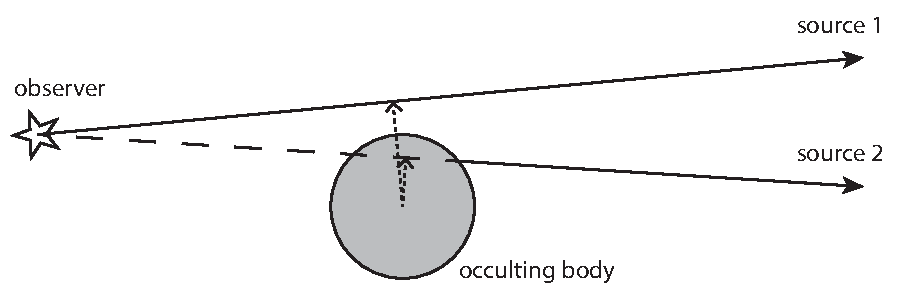
\includegraphics[width=0.7\linewidth]{occult.pdf}
\caption{Simple geometric occultation scheme used in this study. The interception distance (dotted segment) is computed as the distance between the center of the occulting body and the line of sight between the observer and the source. In this case the source 1 is not occulted, while source 2 is.}\label{fig:occult}
\end{figure}


\section{Results} %CL
Figures \ref{fig:flyby_occultation_C30} to \ref{fig:flyby_occultation_I24} present modelling of the occultation. On these four Figures are plotted the GLL/PWS data (same data as in Figure \ref{fig:flyby_data}), together with the simulations of auroral radio emissions (described in Section \ref{sec:ExPRES})) separate into the 4 source types A, B, C and D (from white to black, resp.). The comparison of observations and modelled data shows that the simulations reproduced the Jovian radio occultation during the four flybys presented Figure \ref{fig:flyby_data}, with a few discrepancy in some cases. 

Let's begin with the occultation taking place during the C30 flyby of Callisto displays Figure \ref{fig:flyby_occultation_C30}. The occultation time at ingress is very well reproduced (at one minute accuracy), with all sources occulted simultaneously at the same time where radio emissions intensity drops instantly, at $\sim$~11:25. At egress, we observe first a faint rise of the emission intensity from $\sim$~11:50 to $\sim$~12:00, and then it suddenly returns to its maximum intensity at $\sim$~12:00. This is explained by our simulations, with first the reappearance of 3 types of emission (A, B, C, resp.), and then the fourth emission type (D) at $\sim$~12:00. Regarding the modelling of the low-frequency cut-off, it is not perfectly simulated (especially on the ingress side), with a difference of about $200$~kHz. This lower frequency limit is mostly due to the ratio of the plasma and cyclotron electronic frequencies, which is taken into account in the ExPRES simulations. The error of a few 10s-100S kHz is thus probably due to an incorrect estimation of the electron density around Jupiter (see Section \ref{sec:Discussion} for more details).


In second place comes the E12 Europa's flyby (Fig. \ref{fig:flyby_occultation_E12}). As in the C30 Callisto's flyby case, all sources are occulted simultaneously at ingress. At egress, the simulation well reproduce the end of the occultation, except in the $\simeq$[$800$-$1000$]~kHz frequency range where we observed emission during the modelled occultation. Two physical hypothesis can explain this features. The first one involved reflections effects of the radio emission on the Europa's ionosphere, and the second on reflection inside the Io torus. We will discuss that in more details in Section \ref{sec:Discussion}.

Figure \ref{fig:flyby_occultation_G01} displays the occultation modeling of the Jovian radio emissions during the G01 Ganymede's flyby. At ingress, unlike the previous two cases, all sources are not occulted simultaneously. First the A sources are occulted (we observe a slight intensity decrease in the data), then the B sources (with a second, stronger, intensity decreasing) and finally, almost simultaneously, the southern sources (C and D), with the beginning of the full occultation. At egress, the simulated reappearance of the A sources (white line) well reproduce the end of the observed occultation. Here at both egress and ingress, the radio sources are not occulted simultaneously and at the same time at each frequency, which is due to the trajectory of Galileo \tbd{see movie in the Supporting Information}.


\tbd{BC: choisir un flyby avec occultation, montrer plot et faire film cosmographia en complementary material + screenshot en figure: Pour le film, le cas G01 est pas mal, car on occulte les sources de manière non-simultanée. Il faudrait faire la simulation avec les sources A, B, C et D a plusieurs frequences (e.g. 700 kHz, 1 MHz, 3 Mhz, 5 Mhz) pour bien representer les choses}


Finally, Figure \ref{fig:flyby_occultation_I24} displays the occultation during the I24 Io's flyby. At ingress, the occultation of the higher intensity is well reproduced, due to the occultation by Io's itself. But we still see some radio emission in the data during the modelled occultation probably due to reflection of the radio emission by the Io's ionosphere, no taking into account in our simulations. Moreover, especially at egress, we do not well reproduce the low-frequency cut-off, which is probably due to reflection effect (not simulated here) inside the Io's torus. The Io flyby also shows a noticeable feature. The Northern radio sources (A and B, respectively in white and light-grey) are not observed at the beginning of the studied interval. This is due to the ``Equatorial Shadow Zone'' effect (\tbd{Cecconi et al., 2012}), also reported at Saturn \citep{lamy_JGR_08b}, see Appendix \ref{appendix:esz} for more details. 


%\begin{figure}
%\includegraphics[width=1.0\linewidth]{Moon_flyby_galileo_occultation_data_simu.png}
%    \caption{Superposition of GLL/PWS data and ExPRES simulations during Jovian radio emission occultations by Io (upper left), Europa (upper right), Ganymede (lower left) and Callisto (lower right). \tbd{The four types of emission (A, B, C, D) are separated (from white to dark grey, resp.}.}
%    \label{fig:flyby_occultation}
%\end{figure}

\begin{figure}
    \centering
    \includegraphics[width=0.99\linewidth]{Moon_flyby_galileo_occultation_data_simu_C30.png}
    \caption{Superimposed GLL/PWS data and ExPRES simulations during Jovian radio emission occultations by \object{Callisto} (flyby C30). The four types of emission (A, B, C, D) are separated (from white to dark grey, resp.)}
    \label{fig:flyby_occultation_C30}
\end{figure}


\begin{figure}
    \centering
    \includegraphics[width=0.99\linewidth]{Moon_flyby_galileo_occultation_data_simu_E12.png}
    \caption{Superimposed GLL/PWS data and ExPRES simulations during Jovian radio emission occultations by \object{Europa} (flyby E12). The four types of emission (A, B, C, D) are separated (from white to dark grey, resp.)}
    \label{fig:flyby_occultation_E12}
\end{figure}


\begin{figure}
    \centering
    \includegraphics[width=0.99\linewidth]{Moon_flyby_galileo_occultation_data_simu_G01.png}
    \caption{Superimposed GLL/PWS data and ExPRES simulations during Jovian radio emission occultations by \object{Ganymede} (flyby G01). The four types of emission (A, B, C, D) are separated (from white to dark grey, resp.)}
    \label{fig:flyby_occultation_G01}
\end{figure}




\begin{figure}
    \centering
    \includegraphics[width=0.99\linewidth]{Moon_flyby_galileo_occultation_data_simu_I24.png}
    \caption{Superimposed GLL/PWS data and ExPRES simulations during Jovian radio emission occultations by \object{Io} (flyby I24). The four types of emission (A, B, C, D) are separated (from white to dark grey, resp.)}
    \label{fig:flyby_occultation_I24}
\end{figure}





\section{Usage for the JUICE mission planning tools} %CM+CV

\tbd{Claudio and Claire: fill in this section with what you want to describe.}

The science planning activity, coordinated by the JUICE Science Operations Center, relies on the identification at each point in time of the science observations opportunities, using science models or/and geometry. For JUICE, some of those opportunity periods depend on the Jupiter Radio emission simulation; ionosphere characterization, active and/or passive radar sounding activities opportunities can benefit from an accurate simulation of Jupiter radio emission.

Since the ExPRES Tool can provide as by-product the positions of the radio sources as seen from the spacecraft for a range of frequencies (i.e., 1-40 MHz), the Juice Science Operation Centre (JUICE SOC) has implemented a standalone tool, which wraps the ExPRES tool and identify science opportunity windows based on the radio source position. 

This can be used to identify opportunity windows for one of the high priority science objectives of the Juice RPWI instrument, the icy moon ionosphere characterization through ionosphere refraction/distortion measurement.

The opportunity periods currently generated to drive the corresponding RPWI measurements are linked to the ingress and egress occultation events of the Jupiter Radio Sources, where at least one Jupiter radio sources reach Juice spacecraft with a frequency between 0.1-5 MHz crossing the moon ionosphere (with thickness 0-100km).

In the figure \ref{JUICE SOC-fig1}, the Jupiter auroral radio source as seen from JUICE during 21C13 (the last Callisto flyby of the tour) as a function of frequency (MHz) and UTC time is displayed: the red dots correspond to opportunity for ionosphere characterization, i.e., whenever one of the radio source types (A, B, C or D) is seen by JUICE with a line of sight passing through the ionosphere within 0-100 km. This section is using the CReMA 3.0 trajectory scenario.


\begin{figure}
    \centering
    \includegraphics[width=\textwidth]{sources_C_20320111T173800_20320111T193300_ABCD_periods.png}
    \caption{dots represent the Jupiter auroral radio source state is a function of frequency (MHz) and UTC time for the last Callisto flyby (21C13). Red dots means that at least one of the source type (A, B, C and D) is visible from JUICE and that the line of sight between the source and the spacecraft goes through the ionosphere within 0-100 km altitude above Callisto surface. The blue, orange and green dots mean that no radio source is visible by JUICE at those frequency ranges. Here "No Radio Source" means that there is no emission from the corresponding source; Jupiter ionosphere does not generate emissions at high frequencies while emissions at low frequencies are too weak, and therefore do not produce emissions.}
    \label{JUICE SOC-fig1}
\end{figure}

Figure \ref{JUICE SOC-fig2} shows the resulting ionosphere characterization opportunities as a function of the Juice spacecraft altitude in km (green background). There are a few gaps within the ingress and egress ionosphere characterization opportunities. Those gaps of 1-2 minutes are ignored to compute the final \texttt{iono\_ingress} and \texttt{iono\_egress} envelops used for the observations planning. Table \ref{JUICE SOC-tab1} lists the RPWI in-situ and radio measurement sequence for the 21C13 scenario based on the Closest Approach (CA), and the ingress and egress windows envelope for ionosphere characterization. 

\begin{figure}
    \centering
    \includegraphics[width=\textwidth]{SC_to_Callisto_Distance_C_20320111T173800_20320111T193300_2D.png}
    \caption{Juice spacecraft distance to the Callisto moon surface in km for the 21C13 Flyby (blue line); the Callisto surface (resp. the 1000km altitude above surface) is represented by the red dashed line (resp.\ green dashed line), and the ionosphere characterization opportunities windows are filled in greenish background. }
    \label{JUICE SOC-fig2}
\end{figure}

\begin{table}[]
    \centering
    \begin{tabular}{l|l|r|l|l}
Data time                   & Event	    & Relative Time      & in-situ&radio\\ \hline
\texttt{2032-01-11T05:44:05}&\texttt{CA}&\texttt{$-$12:00:00}& slow	  &full\\
\texttt{2032-01-11T08:14:05}&\texttt{CA}&\texttt{$-$09:30:00}& normal &full\\
\texttt{2032-01-11T17:34:05}&\texttt{CA}&\texttt{$-$00:10:00}& burst  &full\\
\texttt{2032-01-11T17:54:05}&\texttt{CA}&\texttt{$+$00:10:00}  & normal &full\\
\texttt{2032-01-11T17:55:00}&\texttt{iono\_ingress}&\texttt{$+$00:00:00}&normal & burst\\
\texttt{2032-01-11T18:01:00}&\texttt{iono\_egress} &\texttt{$+$00:00:00}&normal & full\\
\texttt{2032-01-11T18:54:00}&\texttt{iono\_ingress}&\texttt{$+$00:00:00}&normal & burst\\
\texttt{2032-01-11T19:11:00}&\texttt{iono\_egress} &\texttt{$+$00:00:00}&normal & full\\
\texttt{2032-01-12T03:14:05}&\texttt{CA}&\texttt{$+$09:30:00}  & slow   &full\\
\texttt{2032-01-12T05:44:05}&\texttt{CA}&\texttt{$-$12:00:00}& slow   &full
    \end{tabular}
    \caption{RPWI in-situ and radio observations mode sequence during the 21C13 \object{Callisto} flyby scenario. Some mode changes are scheduled w.r.t.\ Closest Approach event (CA), while ionosphere characterization observations are scheduled w.r.t ingress and egress events as identified using Express.}
    \label{JUICE SOC-tab1}
\end{table}

Finally figure \ref{JUICE SOC-fig3} is a screenshot of this measurement sequences as shown by the JUICE SOC Mapping and Planning Payload Science software (MAPPS), used to simulate the spacecraft and payload resources status (i.e., power, data rate, on-board solid-stat mass memory (SSMM)). The RPWI operations are planned around the CA and around ingress and egress ionosphere characterization opportunities as described in Table \ref{JUICE SOC-tab1}. The high-resolution in-situ measurement mode is scheduled +/- 10 minutes around the closest approach (CA), while the high resolution radio measurement mode is scheduled during the ionosphere characterization opportunities. High-resolution modes are the more demanding in term of resources (power, data generated, stored in SSMM and to be downloaded (data rate)) and there are reserved for priority scientific objectives. So it is crucial to be able to calculate the corresponding opportunities windows.

\begin{figure}
    \centering
    \includegraphics[width=\textwidth]{21C13_RPWI_Science_timeline_MAPPS.png}
    \caption{This picture is a screenshot of this measurement sequences as shown by the JUICE SOC MAPPS tool, which allows to simulate the spacecraft and science instrument resources status (i.e., power, data rate, on-board memory). The top line is colour coded to reflect the different modes used by RPWI during the sequence. Instrument resources are displayed in the bottom plots. }
    \label{JUICE SOC-fig3}
\end{figure}



The JUICE mission is in development phase, with a planned launch in June 2022. At this stage the JUICE mission science planning process is being exercised by analyzing representative science scenarios similar to 21C13. In this study, the scenario analysis covers +/- 12 hours around the Callisto closest approach.

The JUICE SOC is identifying the same type of opportunity windows whenever a new candidate trajectory is available for JUICE.

The ExPRES tool simulation results can also be useful for other measurement types, and will be made available for by JUICE SOC instrument teams. This includes the measurement linked to the icy shell characterization of the icy moons:
\begin{itemize}
    \item Passive radar measurement by the radar (RIME instrument) or by RPWI: Opportunities can be identified whenever any radio source is visible from the spacecraft for any source type (ABCD), and per source type (to differentiate source from north and south hemisphere) between 1 and 40 MHz (although lower frequencies are better since they have a deeper penetration into the ice);
    \item Active Radar measurement by the radar (RIME instrument): when the spacecraft is protected from Jupiter radio emission due to moon occultation for sources with frequency between 9 and 11 MHz (i.e., flybys and Ganymede phase) and when the spacecraft is within the RIME instrument operating range (altitude <1000km).
\end{itemize}

\section{Discussion} %BC
\label{sec:Discussion}

The Jovian radio emissions are present almost continuously, although this may not be obvious in many observational data sets, due to the limited sensitivity of instruments. Ground based radio telescopes (such as the Nan\c cay Decameter Array in France) provide the longest observation collections, but the distance to Jupiter limits the detection of lower intensity events despite their intrinsic sensitivity. Space borne radio instruments (such as Voyager/PRA, Cassini/RPWS, Galileo/PWS or Juno/Waves), provide observations from a closer distance to Jupiter. Cassini and Galileo data show quasi-continuous radio signals (as shown on Figure \ref{fig:cas-gll-continuous-radio}). The JUICE/RPWI and RIME instruments will observe similar radio signal levels. It is noticeable that the JUICE/RIME and Cassini/RPWS instruments have similar antenna characteristics, leading to an antenna resonance at about $\sim$9 MHz \citep{zarka_JGR_04, Bruzzone:2013ge}. It is thus very likely that JUICE/RIME will observe similar signals as those shown on Figure \ref{fig:cas-gll-continuous-radio} (with a spectral range restricted around 9 MHz). 

At the lower frequencies (e.g., below $\sim$ 1 MHz), the ExPRES code may not provide accurate results, since it doesn't take into account refraction effects. Refraction effects are observed in this frequency range, with the so-called attenuation lanes \citep{gurnett_GRL_98a} resulting from the propagation of hectometric waves through the Io torus plasma \citep{menietti_PSS_03}. These attenuation lanes are observed as a  narrow-band attenuation feature modulated at the planetary rotation period. It is partially visible on both panels of figure \ref{fig:cas-gll-continuous-radio}, between $\sim$ 1 MHz and $\sim$ 3 MHz, as a faint attenuated sinusoidal signature with a period of about 10 hours. However, the low frequency limit is well predicted by ExPRES, as shown on Figures \ref{fig:flyby_occultation_C30} to \ref{fig:flyby_occultation_I24}. The ExPRES low frequency emission limit is determined by the CMI theory: the emission can occur only when $f_p/f_c < 0.01$. This finding implies that our modeling of the magnetic field and plasma density is consistent with the radio observations. 

It is noticeable that faint emissions are still visible during some occultations (e.g., during the E12 and C30 Galileo flybys). This could be resulting from refraction effects in the moon ionosphere. This hypothesis will be investigated in a future study, coupling a ray-tracing code \citep{Gautier:2013uh} with the ExPRES simulation runs. The I24 flyby also shows a mismatch between the observed and predicted occultation (especially during egress). Several effects can occur here. The observer is inside the Io Torus, and thus propagation effects must be taken into account. 

\tbd{Effects due to location: radio sources not observed (or well constrained by model)}


Il faut occulter les 4 sources pour \^etre sur d'\^etre clean. 

The current occultation prediction accuracy is estimated at about 1 minute. This accuracy is based on the GLL/PWS occultation prediction versus observation timings. A more detailed evaluation of this accuracy is not beyond the scope of this study.  


Current sheet model may be updated in future, JRM09 magnetic field model should be accurate enough for our model.



\subsection{Effect of source locations on the occultation}
Figure \ref{fig:compa_mshell_50_30} displays the occultation of the Jovian radio sources during the flyby I24, for two different simulation games. In the top panel, the sources are positioned on the magnetic field lines whose M shell is 50, while in the bottom panel, the sources are positioned on magnetic field lines with an M shell of 30. We can see that there is no difference for the occultation interval. The difference in the low cut-off frequency of the simulated emissions is very small (with a slightly lower low cut-off frequency for sources with M shells of 50). The main difference is observed for the A and B sources (white and light-grey curve). As discussed previously, this feature is due to the equatorial shadow zone (see Appendix \ref{appendix:esz}), a region near the equator where some of the radio emission are not visible anymore, due to the radio emission beaming pattern, along the edges of a hollow cone. Changing the position of the sources implies to (slightly) change the direction of the radio waves, which implies a change in the equatorial shadow zone size.



\begin{figure}
    \centering
    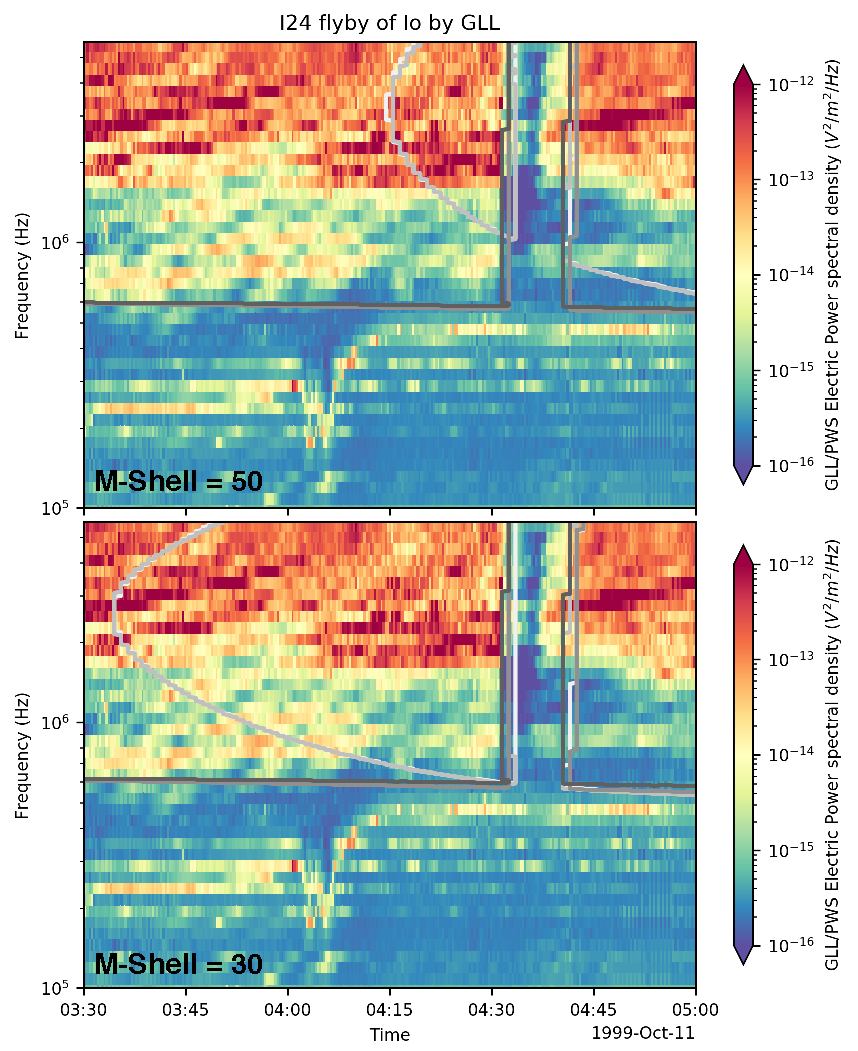
\includegraphics[width=\textwidth]{Moon_flyby_galileo_occultation_data_simu_I24_mshell30-50-compa.pdf}
    \caption{Comparison between the jovian radio occultation during the I24 flyby for sources on magnetic field lines at M shell M=50 (top panel) and M=30 (bottom panel).}
    \label{fig:compa_mshell_50_30}
\end{figure}

\subsection{Refraction effect}
 In Figures \ref{fig:flyby_occultation_C30} to \ref{fig:flyby_occultation_I24} we saw that some faint emissions are visible during the occultation interval, not reproduce by the simulations. The fact that we observe emissions during the interval where the spacecraft is behind the moon, which occults all radio sources, is probably due to refraction effect, either in the moon's ionosphere, in the Io plasma torus or in the plasma sheet. In our simulations, the emissions propagate straight line once emitted, implying that tese refraction effects are not taking into account.
  
 For example, during the E12 Europa's flyby (Fig. \ref{fig:flyby_occultation_E12}), the emission seen during the occultation at $\sim 1$~MHz, are probably due to reflection effect of the radio emission on a plasma structure (Europa's ionosphere or plasma sheet). In our simulation, we do not take any ionosphere and reflection effect, only the body's radius. Ionosphere density estimation: reflection effect when $f_{emission}=f_{pe}$, with $f_{pe}=\sqrt{n_e \times e^2 /m_e / \epsilon_0}/2/\pi$, where $n_e$, $e$ and $m_e$ the electron density, charge and mass respectively, and $\epsilon_0$ the vacuum permitivity. thus here, $n_e=8000-12400$~cm$^{-3}$, which is on agreement with the results obtain by \citep{Kliore_1997_Science} of an electron density of nearly $10^3$ per cubic centimeter.

\tbd{discuter les 2 hypothèses de lieu de réfaction: Ionosphère EUrope ou Tore de Io}

\section{Conclusions and Perspectives} 

Further analysis with ionosphere model of Galilean moons.

Updated current sheet model

\section*{Acknowledgments}

autoplot, das2, uws, 

\appendix
\section{Equatorial Shadow Zone}
\label{appendix:esz}
In the equatorial region, in the innermost magnetosphere, the auroral radio sources are not visible, due to combination of the shape of the radio emission beaming patterns and the topology of the magnetic field lines bearing the radio source. This effect is named ``Equatorial Shadow Zone'' (ESZ). This effect has been identified at Saturn \citep{lamy_JGR_08b}, using a preliminary version of the ExPRES code. It has also been observed at Earth \citep[see, e.g.,][Figure 1]{morioka:insu-01180185}, but not explicitly described.

Our simulation runs show that some of the Jovian auroral radio sources are not always visible at the distance of Io's orbit. Figure \ref{fig:esz-io} shows the observability for each auroral radio source for an observer located on Io's orbit, during one rotation of Jupiter. The simulation shows that the Southern radio sources (namely, the C and D source) are not visible in the CML range 180 to 210 degrees. The Northern radio sources (namely, the A and B source) are observable from all CML, with a drastically reduced spectral range at a CML of about 25 degrees. Since the ESZs do not occur at the same time, an observer will not experience a full dropout of radio signals, as observed at Saturn. 

\begin{figure}
    \centering
    \includegraphics[width=\textwidth]{esz-io.png}
    \caption{Jovian auroral radio source observability from Io's orbit.}
    \label{fig:esz-io}
\end{figure}

\bibliographystyle{aa}
\bibliography{juice-expres}
\end{document}
